\section{讲解笔记：【第5次作业笔记】 静定桁架(1)}
\begin{analysisbox}
本节按题目、答案和讲解笔记顺序整理。对扫描图中的结构几何关系，正文保留 OCR 可识别文字，并在图形页中保留清理后的题图，便于核对杆件、支座、荷载和尺寸。
\end{analysisbox}
\subsection*{第 1 页转写}
桁架作业及答案

即便题目没有强调，也是不包括支座连杆的。

2-23

图2-140所示桁架中零杆的数目为（不包括支座链杆）（C）。（中南大学

2010)

A.6根

B. 7根

C.8根

D.9根

Fp

2+2 +1+2+I

图2-140

两杆结点上无外力作用时

，则两杆均为零杆。

2-24

计算图2-141所示桁架中1、2杆件的轴力。（重庆大学2010）

Emo=0, Fm2+ 2l +hxl20

图2-141
\begin{figure}[H]\centering
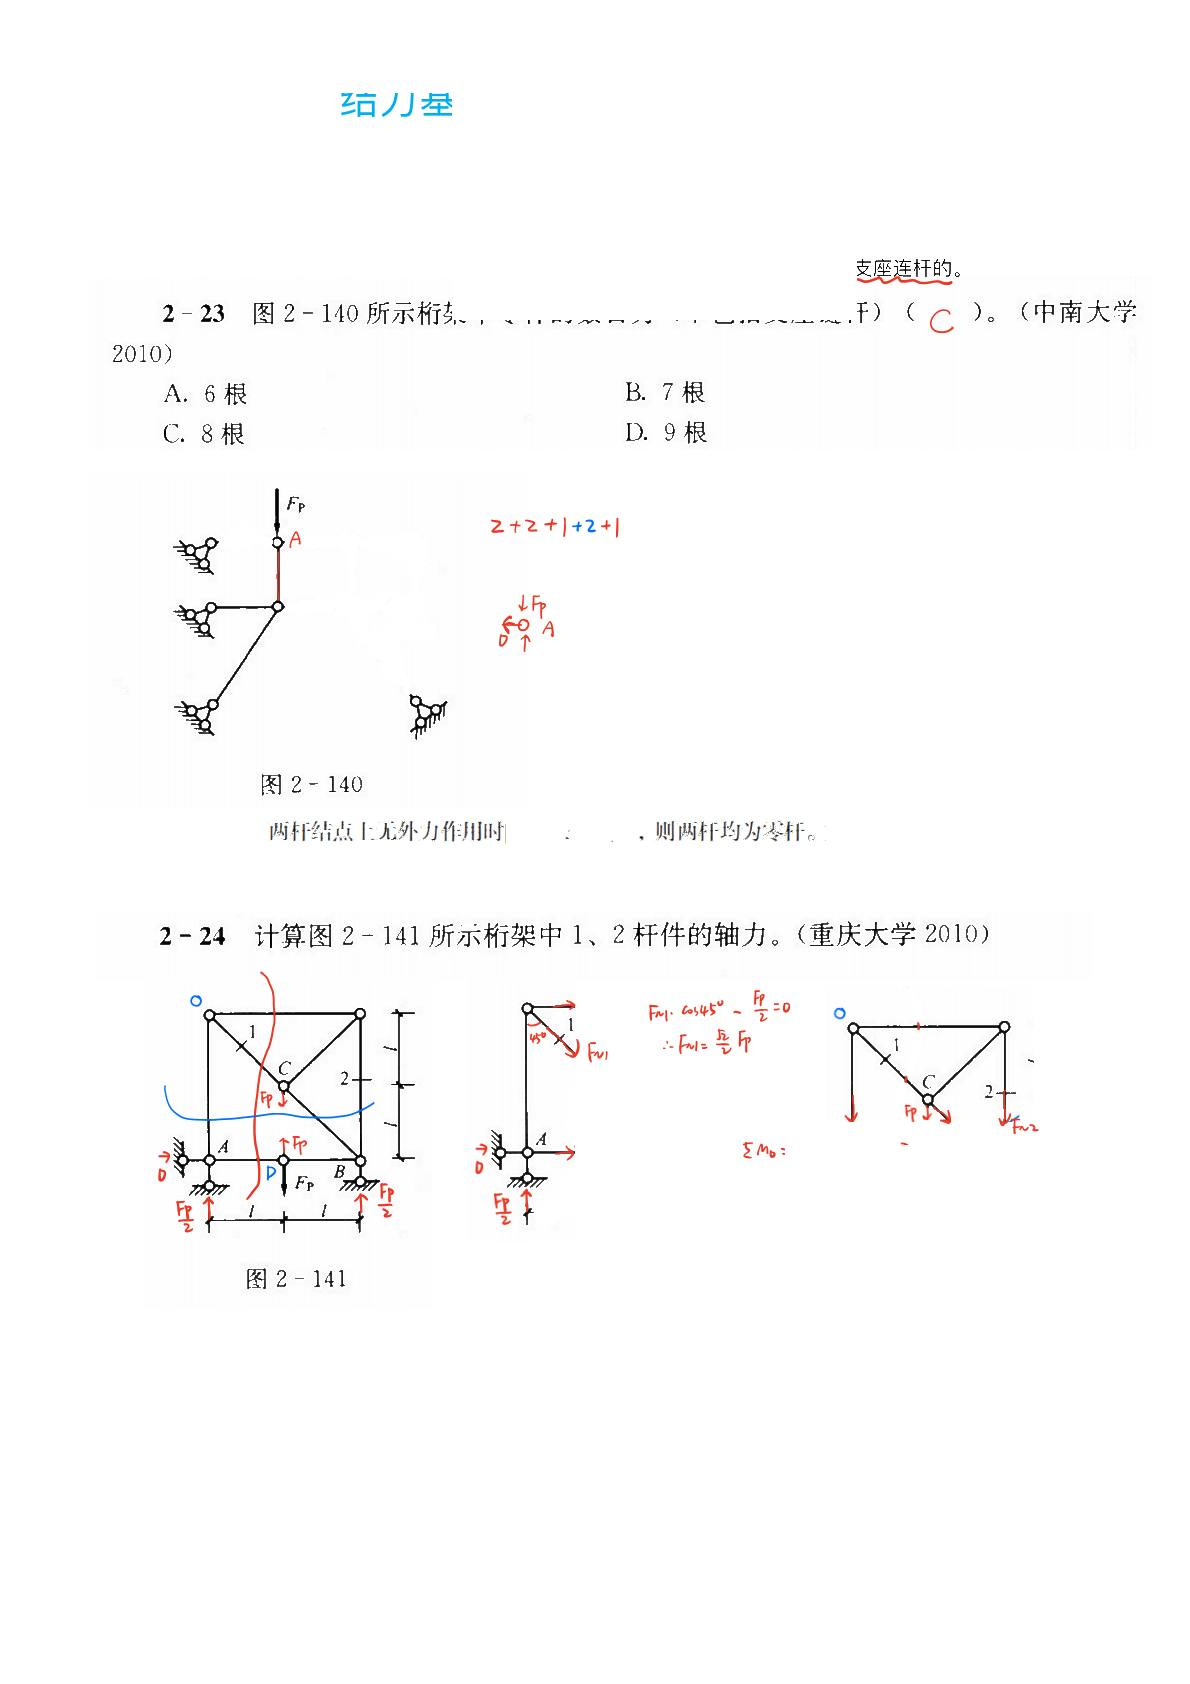
\includegraphics[width=0.92\textwidth]{figures/src25_p001.jpg}
\caption{【第5次作业笔记】 静定桁架(1) 第 1 页清理图形页}
\end{figure}
\subsection*{第 2 页转写}
2-25

50kN

30kN

50kN

30kN

Ix=o, 50+ Fy=0 . Ful= -5okn

Fml0.

图2-142

Sing=

2-Fm. +2-Fnz -0

Fn2: (50): -2

2 -26

求图2-143所示结构中指定杆件1、2的轴力。（广州大学2008）

FL2-CoSD

Fp

Fp

图2-143

ZmA=D,

Fm2

0 =7 - 1x - 1$\times$

FnSmb

Fp

Fp

-2h=0,
\begin{figure}[H]\centering
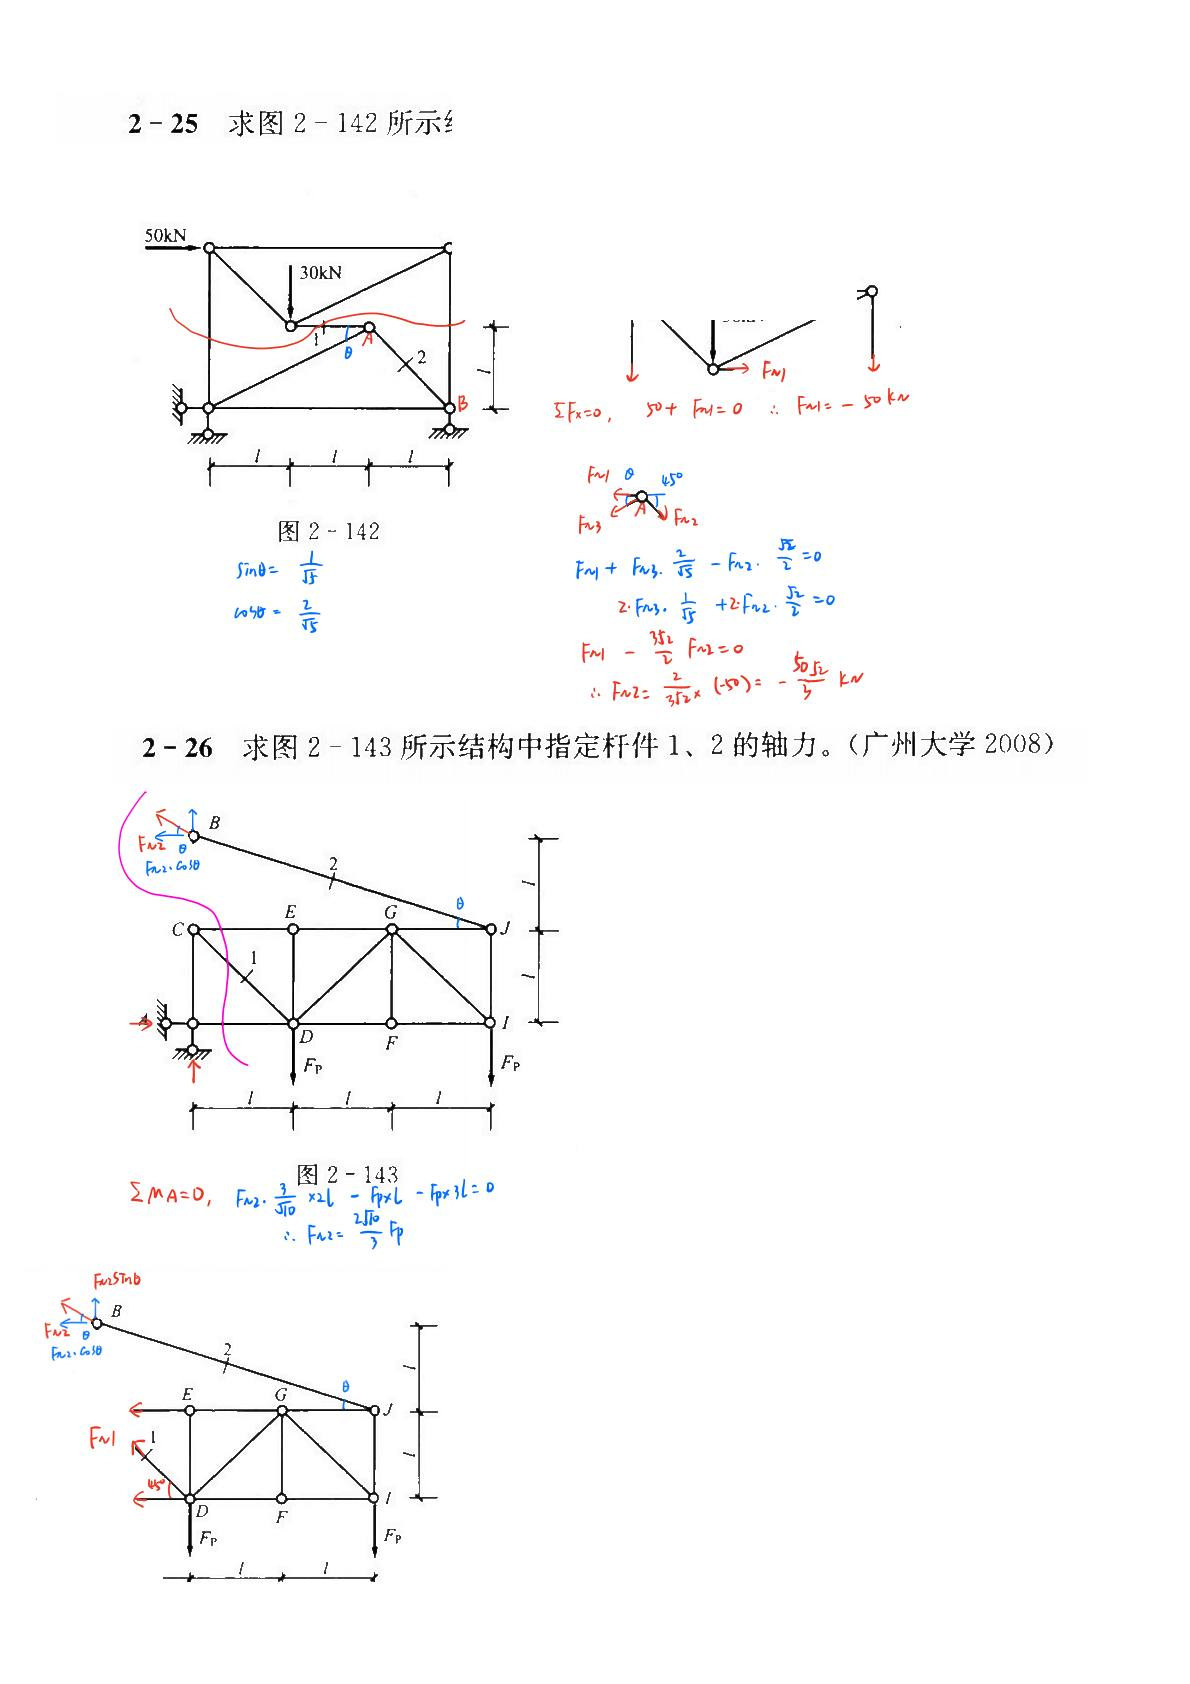
\includegraphics[width=0.92\textwidth]{figures/src25_p002.jpg}
\caption{【第5次作业笔记】 静定桁架(1) 第 2 页清理图形页}
\end{figure}
\subsection*{第 3 页转写}
2 - 27

求图2-144所示桁架中1、2杆的轴力。（西南交通大学2008）

FIA

2Fp

图2-144

Z mB2D

Fyx 4d + 2hpx 2d = hxd + Fpx 3q

.. Fy4= 0

.Fm-0,

2-28

作图2-145所示桁架中a、6、c杆轴力。（西南交通大学2010）

FP

FNE

Fra+ Fp*

.. Fng=-p

图2-145

Frex u -Fxy - Fuax

FP

fux xd - Fux d=0

"Frb:

Fhb
\begin{figure}[H]\centering
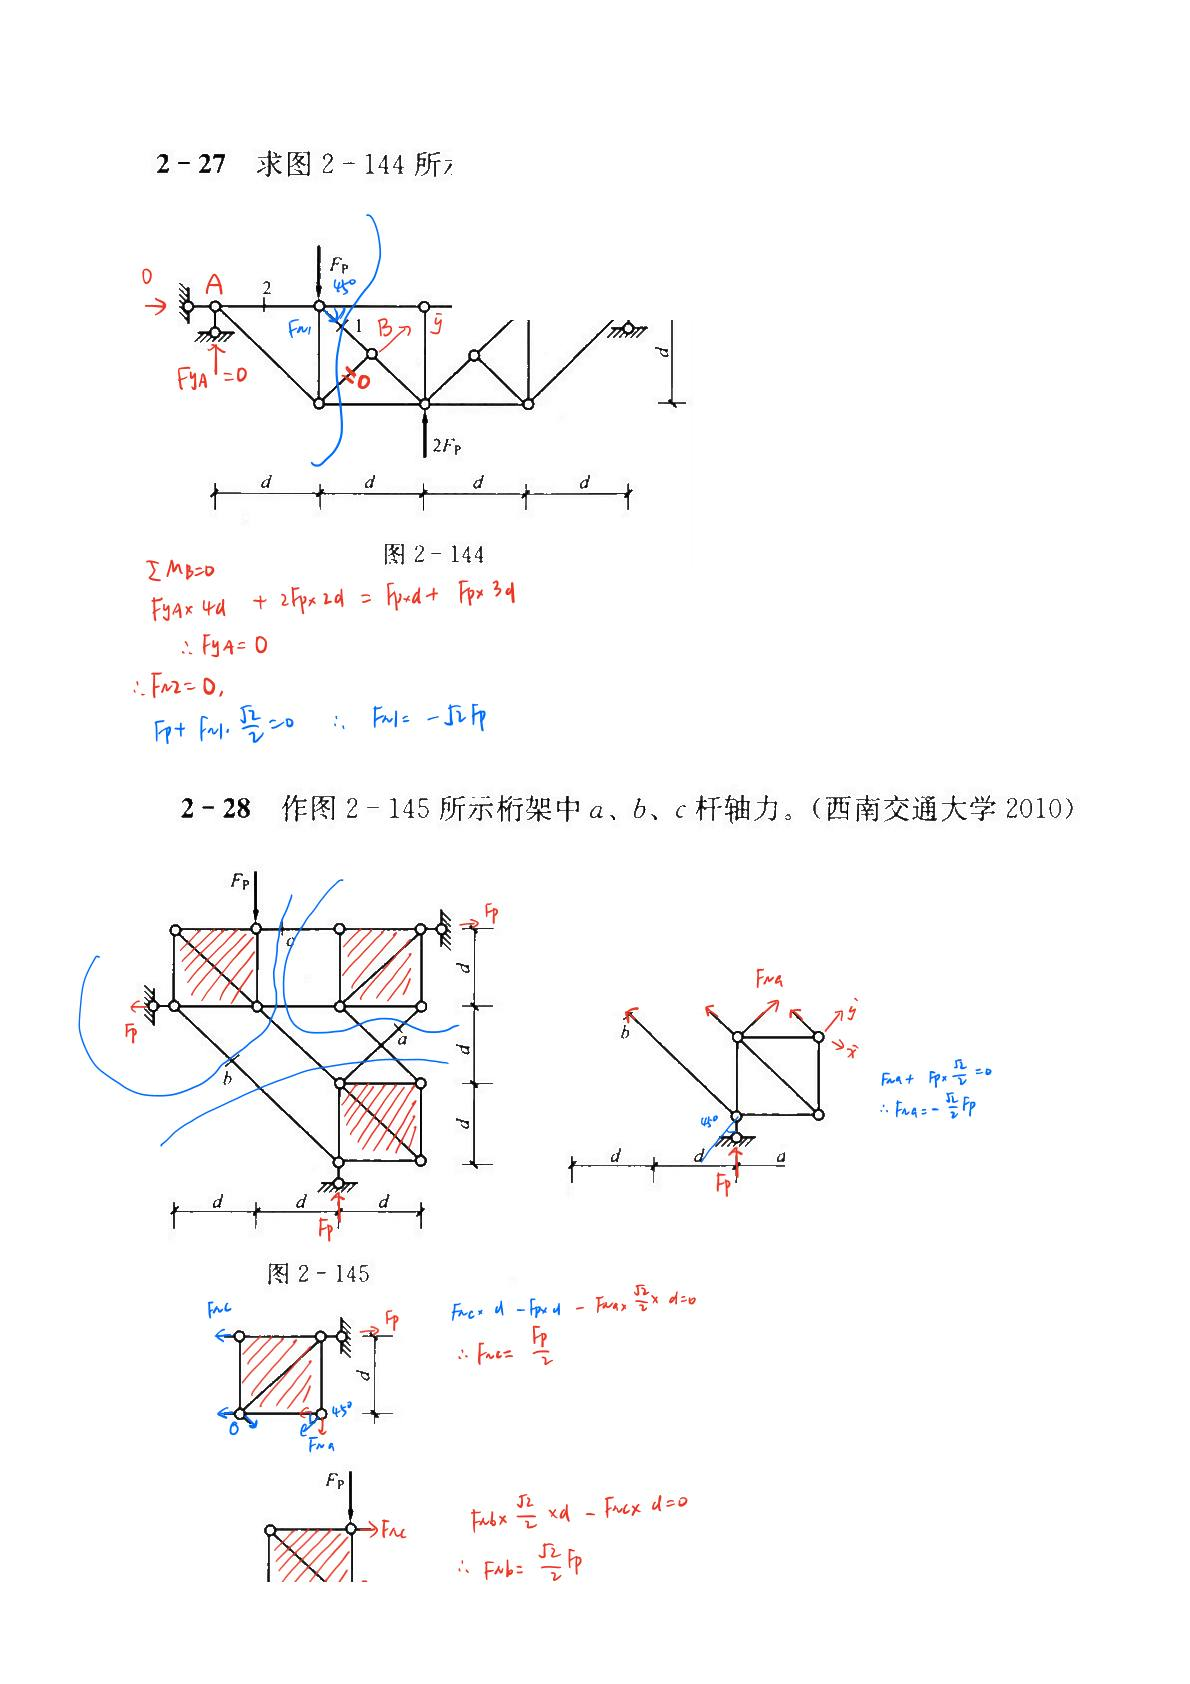
\includegraphics[width=0.92\textwidth]{figures/src25_p003.jpg}
\caption{【第5次作业笔记】 静定桁架(1) 第 3 页清理图形页}
\end{figure}
\subsection*{第 4 页转写}
2-29

试求图2-146所示桁架中a、6杆件的内分。（东北天学2007)

FP

2d

2d

FA

" Fnb-

图2-146

Imb=0,

Fpx2d +F54x 2d -pxu=0, F5A=

IMB=0

Fras-Fp

2-30

求图2-147所示桁架中a、6杆件的内力。（北京航空航天大学2008）

6x

FN4=0

图2-147

Fub:

FA
\begin{figure}[H]\centering
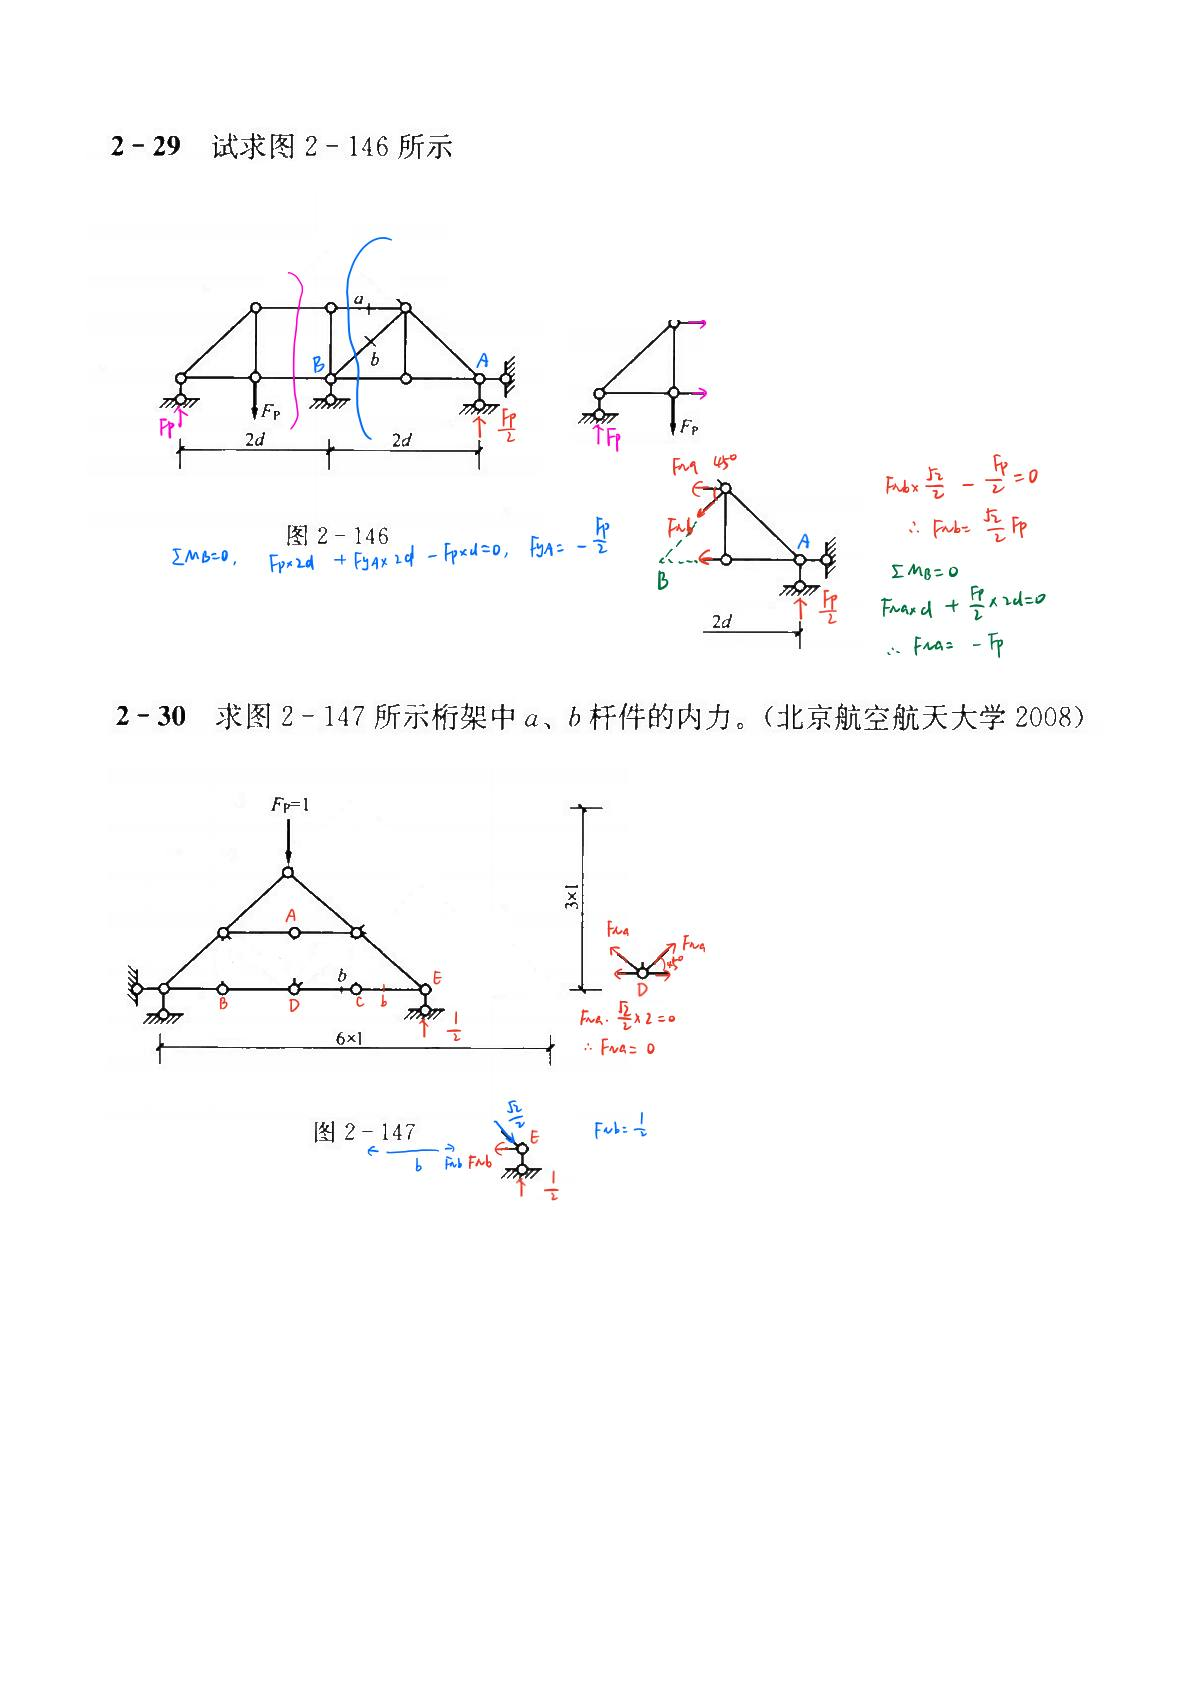
\includegraphics[width=0.92\textwidth]{figures/src25_p004.jpg}
\caption{【第5次作业笔记】 静定桁架(1) 第 4 页清理图形页}
\end{figure}
\subsection*{第 5 页转写}
E

Enb Fp

Fp

D

C

B

A

 ttinaxft

To

i Fna

听

EFnfpFNcihi.fi

fief

嘅

吣 二印

i FnBE  Fp

Fnz

印

在吐8点why

后以前2

1元

in

 

剧

剧卡xz

Fnkoi.FM

可历
\begin{figure}[H]\centering
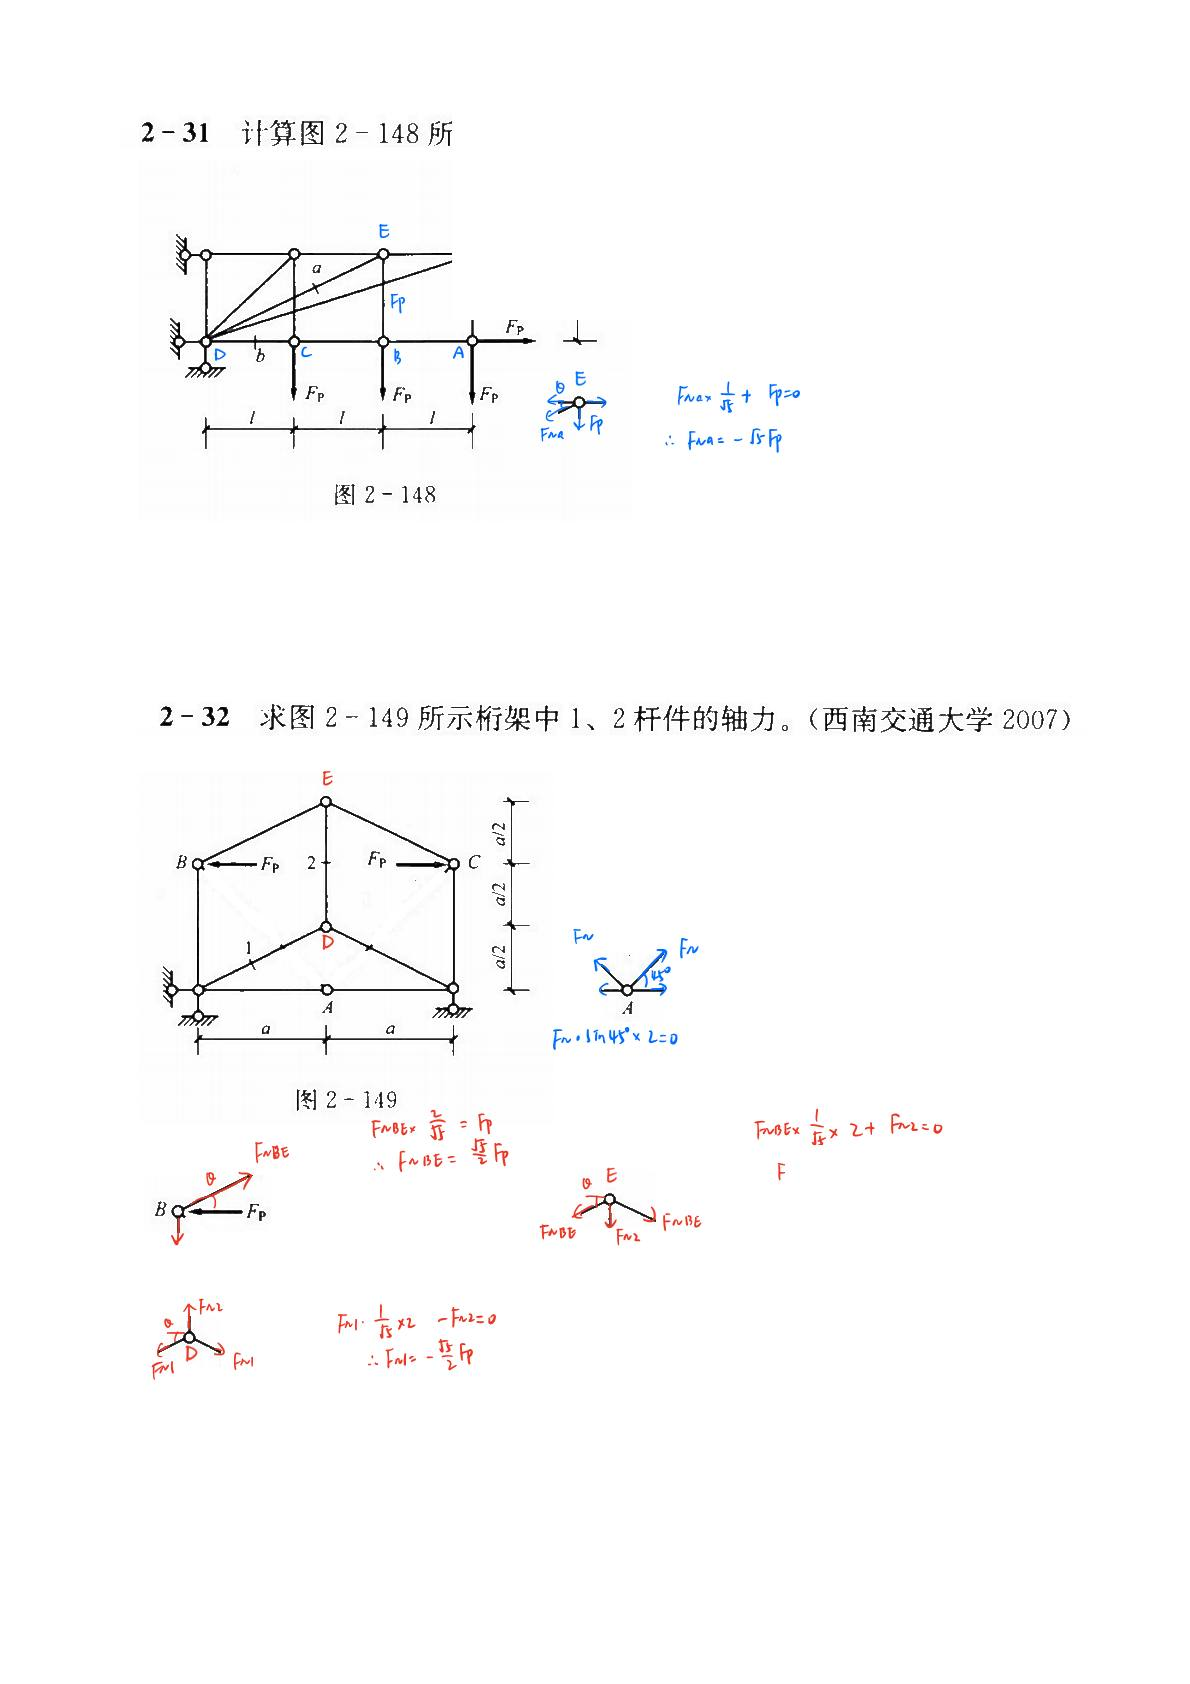
\includegraphics[width=0.92\textwidth]{figures/src25_p005.jpg}
\caption{【第5次作业笔记】 静定桁架(1) 第 5 页清理图形页}
\end{figure}
